\begin{figure}[p]\centering
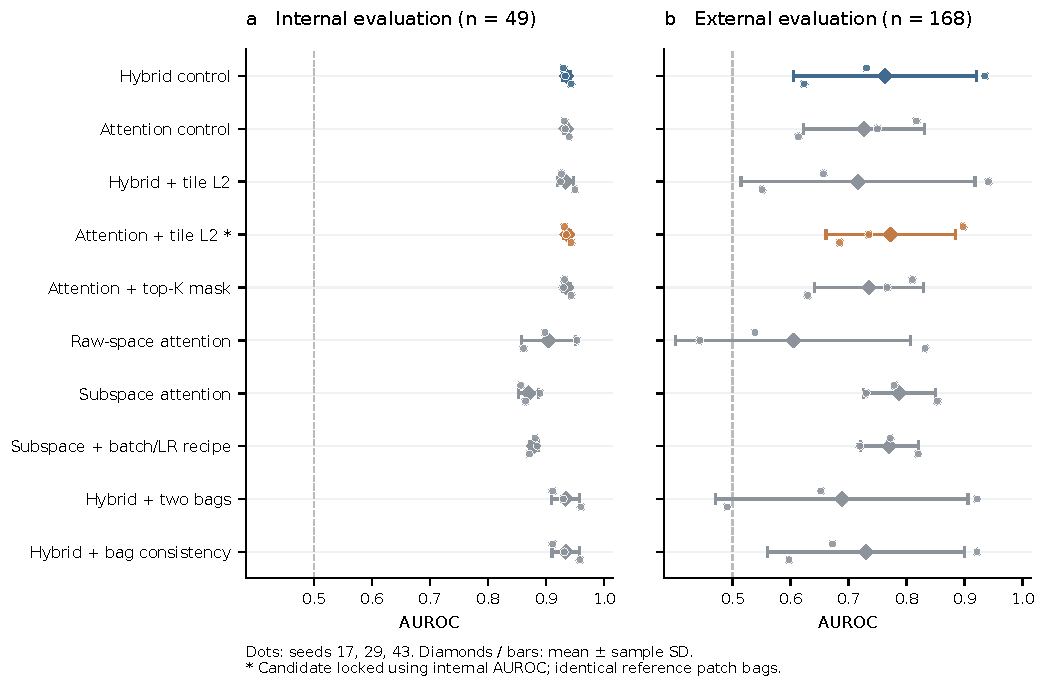
\includegraphics[width=\textwidth,height=.73\textheight,keepaspectratio]{figures/Figure_A1_all_configurations.pdf}
\caption{\textbf{Complete algorithm screen.} All ten configurations and all initial seeds (17, 29, 43) are shown for validation and external evaluation. Individual points are separately trained models; bars summarize mean and sample SD, not confidence intervals. Attention+L2 was selected on mean validation AUROC before external inference. Each cohort contains the same 49 or 168 slides across configurations.}
\end{figure}
\begin{figure}[p]\centering
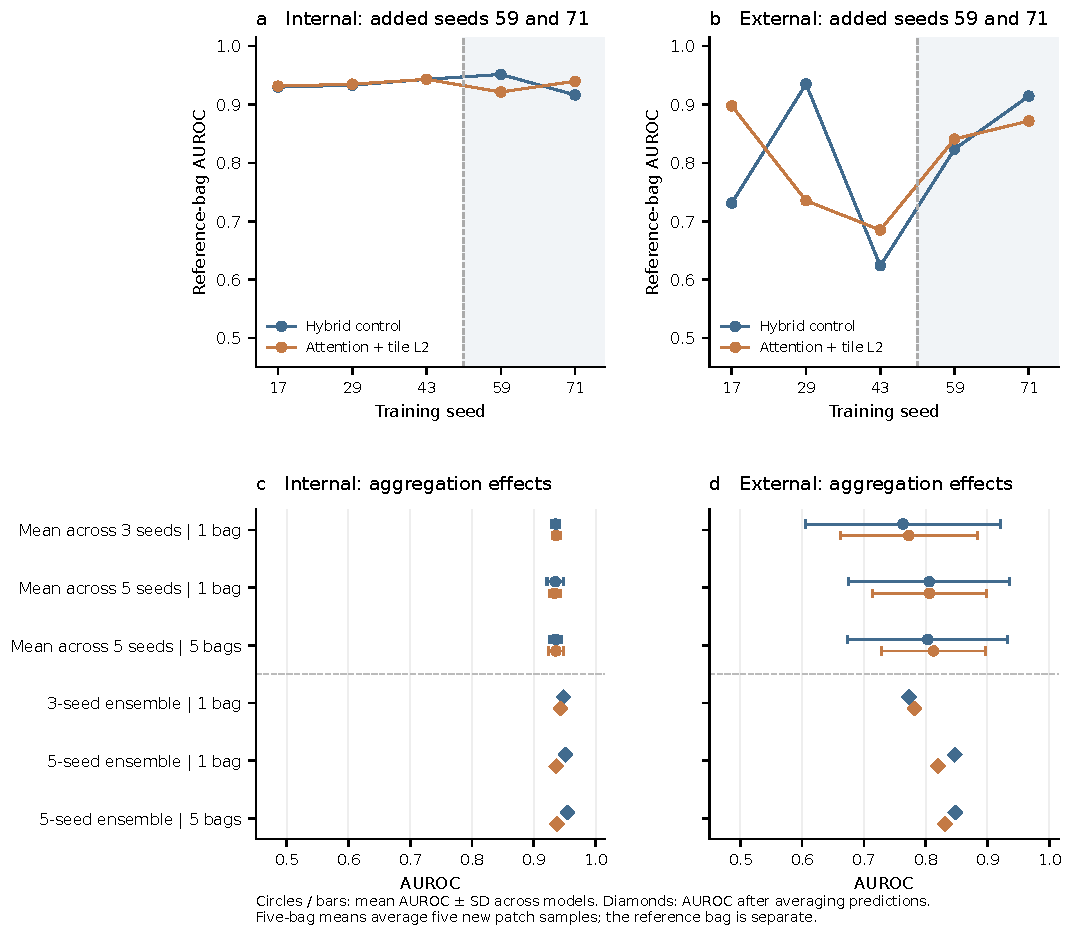
\includegraphics[width=\textwidth,height=.73\textheight,keepaspectratio]{figures/Figure_A2_stability_and_aggregation.pdf}
\caption{\textbf{Training seeds and probability aggregation.} The top panels show all five seeds for the selected candidate and Hybrid; shaded regions identify seeds 59 and 71. Lower panels distinguish mean AUROC across fitted models (circles and SD bars) from AUROC after averaging their probabilities (diamonds). Five-bag means use five new inputs and exclude the reference bag. No seed was omitted.}
\end{figure}
\begin{figure}[p]\centering
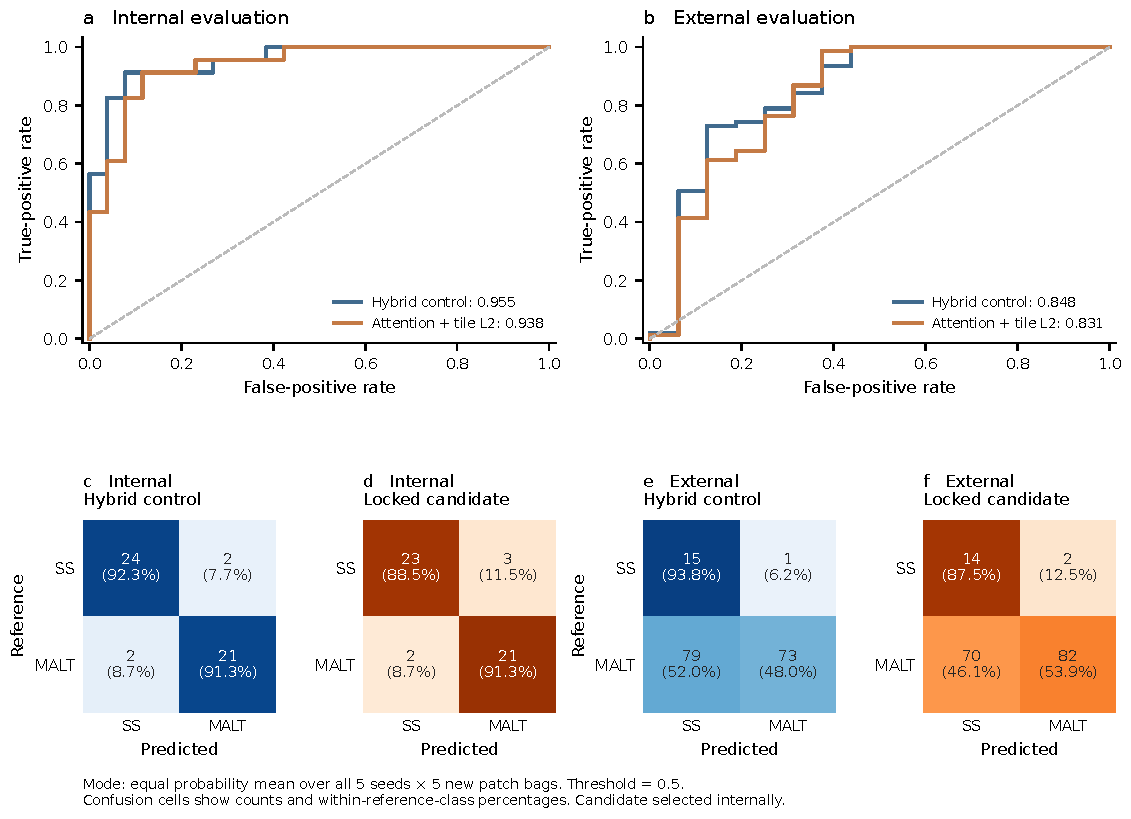
\includegraphics[width=\textwidth,height=.73\textheight,keepaspectratio]{figures/Figure_A3_locked_ensemble_ROC_confusion.pdf}
\caption{\textbf{Five-seed, five-bag probability ensembles.} All 25 probabilities per slide were averaged for each model before calculating ROC and threshold metrics. Confusion matrices use threshold 0.5 and display counts with within-reference-class percentages. These are supplementary development ensembles, not replacements for the retained primary checkpoint.}
\end{figure}
\begin{figure}[p]\centering
\fbox{\begin{minipage}[c][35mm][c]{.88\textwidth}\centering
\textbf{Omitted from this public repository copy}\\[6pt]
This figure contains tissue images or individual-slide observations.\\
The complete figure is retained in the local manuscript archive.
\end{minipage}}
\caption{\textbf{Archived model-region displays for pathological review.} Four cases represent the four threshold outcomes. Performance and visualization bags differed; paired scores for all 12 cases are in Table~S9. Colors represent within-slide-normalized latent-bank margins, not verified MALT/SS labels. The eight displayed crops retain their source pixels, with 50-$\mu$m bars. The false-negative case has unresolved legacy overlay geometry and a low-mask-coverage window, detailed in Supplementary Methods. These displays are retained as review material; they do not establish disease localization or explain errors.}
\end{figure}
\begin{figure}[p]\centering
\fbox{\begin{minipage}[c][35mm][c]{.88\textwidth}\centering
\textbf{Omitted from this public repository copy}\\[6pt]
This figure contains tissue images or individual-slide observations.\\
The complete figure is retained in the local manuscript archive.
\end{minipage}}
\caption{\textbf{Supplied histological context images.} These illustrative MALT and SS images are distinct from the model-selected regions and were not used as regional ground truth. Original pixels are unchanged. Specimen linkage, physical calibration and final descriptions remain completion item H06; no new physical scale is inferred.}
\end{figure}
